%===============================================================================
% Zentrale Layout-Angaben und Befehle
%===============================================================================
%
% Für bessere Sicht von falschen Umbrüchen die Option draft benutzen.
% Dadurch können aber die eingebundenen Bilder nicht sichtbar sein.
\documentclass[a4paper, 12pt]{article}
%
% Hier zunächst die benötigten Packages
\usepackage{german}
\usepackage[utf8]{inputenc}
\usepackage{fancyhdr}
\usepackage[T1]{fontenc}
\usepackage{ae}
\usepackage{listings}
\usepackage{color}
\usepackage{wrapfig}
\usepackage[printonlyused]{acronym}
\usepackage{url}
\usepackage[hypertexnames=false]{hyperref}
\usepackage{fmtcount}
\usepackage[section]{placeins}
\usepackage{tabularx}
\usepackage{amsmath}
\usepackage{nameref}
%
% Einbindung des Grafik-Pakets
\ifx\pdfoutput\undefined
	\usepackage[dvips]{graphicx}
\else
	\usepackage[pdftex]{graphicx}
\pdfcompresslevel=9
\pdfpageheight=297mm
\pdfpagewidth=210mm
\fi
\usepackage[colorinlistoftodos,prependcaption,textsize=tiny]{todonotes}
%
% Page-Layout
\setlength\headheight{14pt}
\setlength\topmargin{-15,4mm}
\setlength\oddsidemargin{-0,4mm}
\setlength\evensidemargin{-0,4mm}
\setlength\textwidth{160mm}
\setlength\textheight{252mm}
%
% Absatzeinstellungen
\setlength\parindent{0mm}
\setlength\parskip{2ex}
%
% dont break math space
\binoppenalty=10000
\relpenalty=10000
%
% Kopf- und Fusszeile
\pagestyle{fancy}
\fancyhf{} % alles löschen
\fancyhead[LO]{\footnotesize\sc\nouppercase{\leftmark}}
\fancyfoot[LO]{\footnotesize\sc Lehrstuhl f\"ur Praktische Informatik}
\fancyfoot[RO]{\thepage}
\renewcommand{\headrulewidth}{0pt}
\renewcommand{\footrulewidth}{0pt}
%
% Bessere Fehlermeldungen
\errorcontextlines=999
%
% Anweisung zur Erstellung der Titelseite
% #1 Bachelorarbeit || Masterarbeit
% #2 = Studiengang
% #3 = Titel der Arbeit
% #4 = Autor
% #5 = Abgabedatum
\renewcommand{\maketitle}[6]
{
\pagenumbering{Alph}
\begin{titlepage}
\centering
\begin{minipage}[t]{16cm}
\begin{minipage}{3cm}
    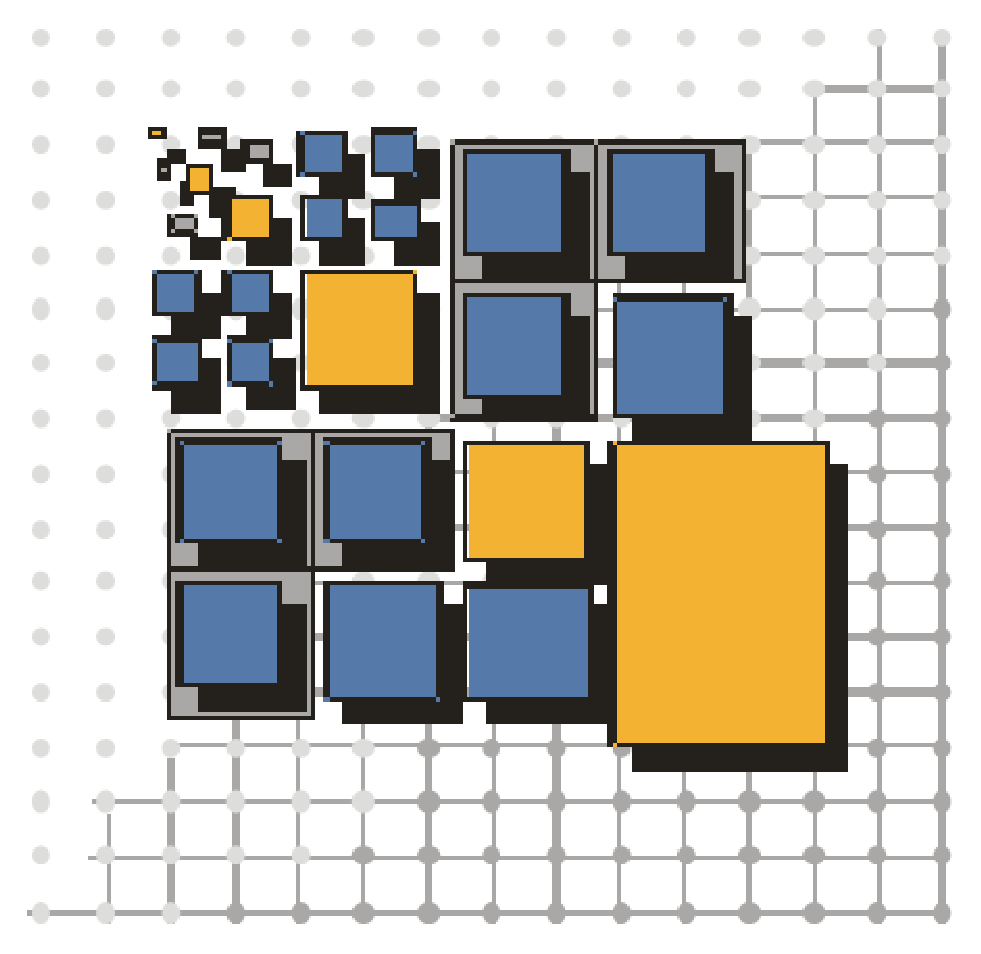
\includegraphics[height=26mm]{includes/vs-logo}
\end{minipage}
\hfill
\begin{minipage}{9cm}
  \centering
    Otto-Friedrich-Universit\"at Bamberg\\[12pt]
    {\Large Lehrstuhl f\"ur Praktische Informatik}
\end{minipage}
\hfill
\begin{minipage}{3cm}
    
\includegraphics[height=26mm]{includes/UB-Logo-neu_blau-cmyk}
\end{minipage}
\end{minipage}\\[130pt]
{\LARGE #1}\\[124pt]
Zum Thema:\\[24pt]
{\Huge #2}\\[60pt]
\vfill
\begin{minipage}{\textwidth}
\center
Vorgelegt von:\\
{\Large #3\\[12pt]}
Betreuer:\\
{#5\\[12pt]}
Themensteller:\\
#6\\[12pt]
Abgabedatum:\\
#4\\
\end{minipage}
\end{titlepage}
}

%
% Wird für Hintergrund von Codelistings benötigt
\definecolor{hellgrau}{gray}{0.9}
%
\lstdefinelanguage{JavaScript}{
	keywords={typeof, new, true, false, catch, function, return, null, catch, switch, var, if, in, while, do, else, case, break},
	ndkeywords={class, export, boolean, throw, implements, import, this},
	sensitive=false,
	comment=[l]{//},
	morecomment=[s]{/*}{*/},
	morestring=[b]',
	morestring=[b]"
}
% Einstellungen für Java-Code
\lstdefinestyle{javaStyle}{%
	basicstyle=\small,%
	backgroundcolor=\color{hellgrau},%
	keywordstyle=\bfseries,%
	showstringspaces=false,%
	numbers=left,%
	numberstyle=\footnotesize,%
	stepnumber=1,%
	numbersep=3pt,%
	extendedchars=true,%
	xleftmargin=2em,%
	lineskip=-1pt,%
	tabsize=4,%
	language=Java,
	breaklines,%
	identifierstyle=\ttfamily,
}
% set default to java, explicitly set to others when needed
\lstset{style=javaStyle}
%
% neues environment für Java-Sourcecode
% #1 = "caption={Hier eigene Überschrift}, label={Hier eigenes Label}"
\lstnewenvironment{javacode}[1][]{%
\lstset{style=javaStyle,#1}%
}{}
%
% Befehl zum Einbinden von Java-Sourcecode aus Datei
% #1 = Dateiname relativ zu src-Verzeichnis
% #2 = Überschrift
% #3 = Label
\newcommand{\javafile}[3]{%
   \lstinputlisting[%
     caption={#2},%
     label={#3},%
     style=javaStyle,
     captionpos=b]{src/#1}%
}
%
% Einbindung eines Bildes
% #1 = Name des Bildes ohne Endung relativ zu images-Verzeichnis
% #2 = Caption
% #3 = label für \ref-Verweise
% #4 = Breite des Bildes im Dokument in % der breite
\newcommand{\asfigure}[4]{%
  \begin{figure}[htb]%
    \begin{center}%
      \includegraphics[width=#4\textwidth]{images/#1}%
      \vskip -0.3cm%
      \caption{#2}%
      \vskip -0,2cm%
      \label{#3}%
    \end{center}%
  \end{figure}%
}
%
% Umgebung für Fliesstext um Grafik
% #1 = Ausrichtung: r, l, i, ...
% #2 = Breite des Bildes in cm
% #3 = Name des Bildes ohne Endung relativ zu images-Verzeichnis
% #4 = Beschriftung
% #5 = label für \ref-Verweise
\newcommand{\textflow}[5]{%
\begin{wrapfigure}{#1}{#2cm}%
\includegraphics[width=#2cm]{images/#3}%
\caption{#4}%
\label{#5}%
\end{wrapfigure}%
}
%%%
\makeatletter
\let\orgdescriptionlabel\descriptionlabel
\renewcommand*{\descriptionlabel}[1]{%
	\let\orglabel\label
	\let\label\@gobble
	\phantomsection
	\edef\@currentlabel{#1}%
	%\edef\@currentlabelname{#1}%
	\let\label\orglabel
	\orgdescriptionlabel{#1}%
}
\makeatother

%%% Local Variables:
%%% mode: latex
%%% TeX-master: t
%%% End:

\usepackage{listings}
%
% Backgroundcolor
\definecolor{hellgrau}{gray}{0.9}
%
% Configuration
%
\lstdefinestyle{javaStyle}{%
	basicstyle=\small,%
	backgroundcolor=\color{hellgrau},%
	keywordstyle=\bfseries,%
	showstringspaces=false,%
	numbers=left,%
	numberstyle=\footnotesize,%
	stepnumber=1,%
	numbersep=3pt,%
	extendedchars=true,%
	xleftmargin=2em,%
	lineskip=-1pt,%
	tabsize=4,%
	language=Java,
	breaklines,%
	identifierstyle=\ttfamily,
}
%
% Java-Sourcecode environment
% #1 = Caption
% #2 = Label
%
\lstnewenvironment{javacode}[2]%
{\lstset{style=javaStyle,caption=#1,label=#2}}
{}
% Include code from Java-file
% #1 = Filename relative to section-folder
% #2 = Caption
% #3 = Label
%
\newcommand{\javafile}[3]{%
   \lstinputlisting[%
     caption={#2},%
     label={#3},%
     style=javaStyle]{src/#1}%
}

%
\begin{document}
%
% Titelblatt erstellen
\maketitle{Thema des Seminars}{Thema Alles LaTeX Oder Was ?}%
{Autor}{Prof. Dr. Guido Wirtz}{Wintersemester 2013}{Bachelor|Master}
%
% Erstellung der Inhaltsverzeichnisse
\pagenumbering{Roman}
\tableofcontents
\newpage
\listoffigures
\newpage
\listoftables
\newpage
\lstlistoflistings
\newpage
%
% Abkürzungen
%
\section*{Abkürzungsverzeichnis}
% In Klammern steht das längste Akronym!
\begin{acronym}[LSPI]
 \acro{DSG}{Distributed Systems Group}
 \acro{LSPI}{Lehrstuhl für Praktische Informatik}
\end{acronym}
\newpage
\setcounter{page}{1}
\pagenumbering{arabic}
%
% Hier einzelne Kapitel mit \input{Kapitel-File} einfügen
%
%
\section{Einleitung}
%
Zur Verfassung von Seminar-, Bachelor- und Masterarbeiten bietet die Distributed Systems Group
neben den Word-Vorlagen auch Vorlagen für Latex. In diesem Dokument soll
kurz gezeigt, wie die einzelnen Umgebungen und Befehle der Vorlage sinnvoll zur Erstellung
von Arbeiten genutzt werden können. Es erfolgt aber keine allgemeine Anleitung zur
Erstellung von Dokumenten mit \LaTeX. Als Einstiegsliteratur, die aber für die allgemeine
Arbeit mit \LaTeX~durchaus ausreichend ist, eignet sich das Buch von Kopka \cite{kop02}. Eines
der älteren Werke des Autors reicht ebenfalls aus. 
Eine sehr gute Übersicht über alle wichtigen Szenarien gibt das Wikibook "`\LaTeX"' \cite{lat12}.
Weitere hilfreiche Lektüre findet sich
unter \cite{jue00}, \cite{kue11}, \cite{jue95}, \cite{erb09} und allen verfügbaren Suchmaschinen.

Die Erstellung eines \LaTeX-Dokumentes erfolgt z.B. über die Anweisung \texttt{pdflatex seminar} oder mit einer 
entsprechenden IDE, wie \textit{TeXnicCenter}\footnote{\url{http://www.texniccenter.org}} oder \textit{TeXlipse}\footnote{\url{http://texlipse.sourceforge.net}}.
Hier empfiehlt sich auch das Zusammenspiel mit SumatraPDF\footnote{\url{http://blog.kowalczyk.info/software/sumatrapdf/free-pdf-reader-de.html}}, das eine Vorwärts- und Rückwärtssuche in den Dokumenten ermöglicht. 
%
%
\section{Genereller Aufbau}
%
Die zentrale Datei der Vorlage ist die Datei \texttt{seminar.tex}, die vom Autor für jeweilige Arbeit
anzupassen ist. In dieser Datei können die Einstellungen für die Titelseite vorgenommen
werden. Des Weiteren müssen in dieser Datei die einzelnen Kapitel der Arbeit, sowie die
\textit{.bib}-Datei mit den \textit{bibtex}-Einträgen eingebunden werden.
%
\subsection{Erstellung einer Titelseite}
%
Die Erstellung der Titelseite erfolgt über den Befehl \texttt{\textbackslash maketitle}. Die Anzahl der Parameter,
mit der dieser Befehl aufgerufen wird, hängt davon ab, ob eine Seminararbeit oder
eine Bachelor-/Masterarbeit erstellt werden soll.
Zur Erstellung einer Titelseite für eine Seminararbeit muss der Befehl \texttt{\textbackslash maketitle} mit
sechs Parametern aufgerufen werden.
%
\begin{verbatim}
\maketitle{Thema des Seminars}{Thema der Ausarbeitung}%
{Autor}{Betreuer}{Semester}{Bachelor|Master}
\end{verbatim}
%
Die einzelnen Paramter sind selbsterklärend. Falls die Seminararbeit von mehreren Autoren
verfasst wird, sind diese durch \texttt{,\textbackslash\textbackslash} zu trennen. Bei drei Autoren ist also z.B. die
Zeichenkette \texttt{Hans Meier,\textbackslash\textbackslash\ Peter Müller und\textbackslash\textbackslash\ Hans Müller} als dritten Parameter
einzusetzen. Als Semesterangabe sollte ein Kürzel wie \texttt{SoSe13} übergeben werden.

Um die Titelseite einer Abschlussarbeit zu erstellen, ist der Befehl \texttt{\textbackslash maketitle} mit drei
Parametern aufzurufen.
%
\begin{verbatim}
\maketitle{Bachelor-/Masterarbeit}{Studiengang}{Thema der Arbeit}%
{Autor}{Abgabedatum}
\end{verbatim}
%
Auch in diesem Fall sind die Parameter selbsterklärend.
%
\subsection{Einbindung der einzelnen Kapitel}
%
Um die Übersichtlichkeit der erstellten Arbeit zu gewährleisten, ist es sinnvoll, für jedes
Kapitel eine einzelne \textit{.tex}-Datei zu erstellen. 
Damit unter Verwendung dieser Dateien ein einzelnes Dokument erstellt wird, sind die einzelnen Kapitel in der Datei \texttt{seminar.tex}
einzubinden. Dies erfolgt über den Befehl \texttt{\textbackslash input}. Soll z.B. ein Kapitel eingefügt werden,
dass in der Datei \texttt{kapitel-1.tex} enthalten ist, so geschieht dies durch die folgende
Anweisung.

\texttt{\textbackslash input\{kapitel-1\}}

Diese Anweisung ist an der in der Datei \texttt{seminar.tex} markierten Stelle einzufügen. 
%
\subsection{Einbindung des Literaturverzeichnisses}
%
Die einzelnen Literaturquellen sind in einer \textit{.bib}--Datei aufzuführen. Die \textit{bibtex}--Datei \texttt{example.bib} enthält einige Beispiele, wie
verschiedenen Quellen wie Buch, Artikel usw. in dieser Datei aufzuführen sind. Jeder der
Einträge benötigt zur Referenzierung ein eindeutiges Label, das sich aus den ersten drei
Buchstaben des Nachnamen des Autors und den letzten beiden Ziffern der Jahreszahl der
Veröffentlichung ergeben. Sind mehrere Autoren bei einer Literaturquelle aufgeführt, so
ergibt sich der Label aus den Anfangsbuchstaben der Nachnamen der ersten drei Autoren
und den letzten beiden Ziffern der Jahreszahl der Veröffentlichung. Falls ein Autor in einem
Jahr mehrere Werke veröffentlich hat, so sind die weiteren Label mit kleinen Buchstaben,
beginnend bei \textit{b}, zu ergänzen.

Eine \textit{.bib}-Datei ist mit Hilfe der Anweisung \texttt{\textbackslash bibliography} in der Datei \texttt{seminar.tex} einzubinden.
Die hier verwendete Datei \texttt{references.bib} wurde also durch durch folgende Anweisung
in dieses Dokument eingebunden.

\texttt{\textbackslash bibliography\{references\}}
%
%
\section{Einbindung von Grafiken}
%
Im Allgemeinen werden Grafiken zwischen Absätzen eingefügt. Eine andere
Möglichkeit ist es, die Grafiken von Text umfließen zu lassen. Generell gilt
aber, dass die Grafiken als \emph{pdf}- oder \emph{eps}-Dateien vorliegen
sollten. Dies hängt davon ab, ob \emph{latex} oder \emph{pdflatex} zur Erzeugung
des Dokumentes verwendet wird. Wird \emph{latex} zur Erzeugung genutzt, so
können nur \emph{eps}-Dateien eingebunden werden. Wird das Dokument mit
\emph{pdflatex} erstellt, so sind \emph{pdf}-Dateien zu verwenden.

Grafiken müssen generell im \emph{images}-Verzeichnis vorhanden sein, um sie
erfolgreich einbinden zu können. Selbst erstellte Grafiken müssen also in das
\emph{images}-Verzeichnis kopiert werden.

\subsection{Grafiken zwischen Absätzen}
%
Eine Einbindung von Grafiken zwischen Absätzen erfolgt mit dem Befehl
\texttt{\textbackslash asfigure}.
\begin{verbatim}
\asfigure{bild1}{vs-logo}{DSG-Logo}{5}
\end{verbatim}
Der erste Parameter \texttt{bild1} dient als Label für Referenzen auf die
Grafik. Der zweite Parameter ist der Name der Grafikdatei ohne Endung. Als
dritten Parameter ist dem Befehl \texttt{\textbackslash asfigure} die Beschriftung
der Abbildung zu übergeben. Der letzte Parameter gibt
die Breite der Grafik in cm an. Die Größenangabe darf aber nur als Zahl erfolgen.
Ist eine Grafik breiter als der übergebene Parameter, so wird sie verkleinert, kleinere Grafiken werden
entsprechend vergrößert. Der obige Befehl führt zu der folgenden Abbildung
\ref{bild1}.

\asfigure{bild1}{vs-logo}{DSG-Logo}{5}

\subsection{Von Text umflossene Grafiken}
%
Sollen Grafiken von Text umflossen werden, so ist der Befehl
\texttt{\textbackslash textflow} zu benutzen. Dieser Befehl basiert auf dem Paket
\emph{wrapfig}, dass u.U. nachinstalliert werden muss. Dieses
\textflow{r}{3}{vs-logo}{DSG-Logo}{bild2}
Paket ist, wie alle anderen Umgebungen mit dieser Funktionalität, etwas
beschränkt und zum Teil fehlerhaft, deshalb ist die Nutzung nur unter Vorbehalt
empfohlen. Eine Grafik kann wie folgt eingebunden werden.\\\\
\verb+\textflow{r}{3}{vs-logo}{DSG-Logo}{bild2}+\\\\
Nach diesem Befehl folgt der Text, der das eingebundene Bild umfliessen
soll. Für den ersten Parameter kommen als einzig relevante Möglichkeiten die
kleinen Buchstaben \emph{l} und \emph{r} in Frage. Diese sorgen für eine
Anordnung der Grafik auf der linken, bzw. rechten Seite. Mit Hilfe des zweiten
Parameters wird die gewünschte Breite der Grafik in cm angegeben, die
entsprechend skaliert wird. Der dritte Parameter ist der Name der Grafikdatei
ohne Endung. Der vierte Parameter bestimmt die Bezeichnung der Grafik. Durch den
fünften Parameter kann ein Label zur Referenzierung angegeben werden.

Eine Eigenheit dieses Pakets ist es, dass Grafiken immer am Anfang eines
Absatzes eingefügt werden. Soll eine Grafik von einem Absatz komplett
umschlossen werden, wie dies bei der Abbildung \ref{bild2} der Fall ist, so ist
der \texttt{\textbackslash fliesstext}-Befehl nicht vor dem Absatz aufzuführen, sondern in
den Text zu integrieren. Der obige \texttt{\textbackslash fliesstext}-Befehl ist demnach
hinter dem Wort "`Dieses"' in den Quelltext eingefügt worden.
%
%
%
\section{Including Java source code}
%
To include Java source code, the package \emph{listings} is required, which might have to be installed.
This package enables the inclusion of source code from various programming languages into the document.
There are two possibilities to include source code in a document. 
One possibility is to put the source code directly in the document and the other is to read it from a file.

To include source code directly, a special environment is required which is shown in the following example:

\begin{verbatim}
\begin{javacode}{This is the first listing}{listing1}
public class Test{

  public Test(){
    // do something
  }

}
\end{javacode}
\end{verbatim}
%
First, an environment called \texttt{javacode} is created.
Required parameters are a caption and a label.
Then follows the actual source code and the environment is closed again.
The above example leads to listing \ref{listing1}.

\begin{javacode}{This is the first listing}{listing1}
public class Test {

  public Test(){
    // do something
  }

}
\end{javacode}

As an alternative, the source code can also be read from a file.
This is beneficial, because it increases the readability.
To include source code from a file, the command \texttt{\textbackslash javafile} is used. 
For a successful inclusion, the source code file has to be located in the \texttt{src}-directory. 

Example usage:
\begin{verbatim}
\javafile{src.java}{This is the second listing}{listing2}
\end{verbatim}

The first parameter has to be the name of the file (with file ending) inside the \emph{src}--directory.
The second parameter defines the caption and the third parameter is the label for referencing the listing.

The above example leads to listing \ref{listing2} as a result.

\javafile{src.java}{This is the second listing}{listing2}
%
%
\section{Nutzung des Abkürzungsverzeichnisses}
%
Zur Einbindung des Abkürzungsverzeichnisses wird das \texttt{acronym}--Package\footnote{\url{http://www.ctan.org/tex-archive/macros/latex/contrib/acronym}} verwendet.
Der Eintrag aller verwendeten Abkürzungen erfolgt in der Datei \texttt{abbreviations.tex}, die bspw. den folgenden Inhalt hat:
%
\begin{verbatim}
	\begin{acronym}[LSPI]
	 \acro{DSG}{Distributed Systems Group}
	 \acro{LSPI}{Lehrstuhl für Praktische Informatik}
	\end{acronym}
\end{verbatim}
%
Die geklammerte Abkürzung \texttt{[LSPI]} sollte dabei durch die längste vorhandene Abkürzung ersetzt werden.
Eine Abkürzung wird mit dem Befehl \texttt{\textbackslash acro} innerhalb der \texttt{acronym}--Umgebung definiert.
Standardmäßig werden nur die im Text tatsächlich verwendeten Abkürzungen auch im Verzeichnis ausgegeben.
Um eine Abkürzung innerhalb eines Textes einzufügen genügt der folgende Ausdruck:

\texttt{\textbackslash ac\{}\textit{<acronym>}\texttt{\}}

Bei der ersten Verwendung innerhalb des Textes bewirkt die Anweisung, dass der vollständige Name gefolgt von der Abkürzung in Klammern ausgegeben wird.
Bei jeder weiteren Verwendung wird lediglich die Kurzform ausgegeben. Die Anweisung \texttt{\textbackslash ac\{DSG\}} erzeugt also zunächst die Langform "`\ac{DSG}"'.
Anschließend nur noch die Abkürzung "`\ac{DSG}"'.
\newpage
%
% Einstellungen für Literaturverzeichnis
\addcontentsline{toc}{section}{\bibname}
\bibliographystyle{IEEEtran}
%
% Hier den bib-file einbinden
\bibliography{bibliography/references}
\end{document}
